\documentclass{article}

\usepackage[utf8]{inputenc}
\usepackage[spanish]{babel}
\usepackage{graphicx}
\usepackage{hyperref}
\usepackage{amsmath}

\graphicspath{ {images/} }

\title{Introducción a la Ingeniería del Software}

\author{Daniel Monjas Miguélez}

\date{\today}

\begin{document}
\maketitle

\newpage

\tableofcontents

\newpage

\section{El producto Software}
\subsection{Naturaleza del software}
La naturaleza del software es dual (como la dualidad onda-partícula en física). Dependiendo de la situación la naturaleza se puede tratar como:

\begin{itemize}
\item Producto.
	
	\begin{itemize}
	\item Proporciona potencial de cómputo.
	
	\item Es un transformador de información.
	\end{itemize}

\item Vehículo, para distribuir un producto.

	\begin{itemize}
	\item Actúa como base para el control de la computadora. Sistemas Operativos.
	
	\item Actúa como base para la comunicación de información. Redes.
	
	\item Actúa como base para la creación y control de otros programas. Herramientas y ambientes de software.
	\end{itemize}
\end{itemize}

El software distribuye el producto más importante de nuestro tiempo, \textbf{la información}.

\subsection{Definición de software}
Cuando se trata al software como un programa de computadora hablamos de una definición incompleta. El software es:

\begin{enumerate}
\item Instrucciones (programas) que cuando se ejecutan proporcionan las funciones características buscadas.

\item Estructuras de datos que permiten a los programas manipular la información adecuadamente.

\item Información en papel o en forma virtual (documentación) que describe la operación y uso de los programas.
\end{enumerate}

\subsection{Características del software.}
\begin{itemize}
\item El software se desarrolla o modifica con intelecto; no se manufactura en el sentido clásico. Aunque hay similitudes entre el desarrollo de software y la fabricación de hardware, las dos actividades son diferentes en lo fundamental. En ambas, la alta calidad se logra a través de un buen diseño, pero la fase de manufactura del hardware introduce problemas de calidad que no existe en el software. Ambas actividades dependen de personas, pero la relación entre los individuos dedicados y el trabajo logrado es diferente por completo. Las dos actividades requieren la construcción de un ``producto'', pero los enfoques son distintos. Los costos del software se concentran en la ingeniería.

\item El software no se ``desgasta'', pero se deteriora. En la figura \ref{tasa_hardware} se ve que el hardware presenta una tasa de fallas elevada en una etapa temprana de su vida (atribuible a defectos de diseño o manufactura); los defectos se corrigen y la tasa de fallas se abate a un nivel estable durante cierto tiempo. Conforme pasa el tiempo, la tasa de fallos aumenta de nuevo a medida que los componentes hardware resienten los efectos acumulativos de suciedad, vibración, abuso, temperaturas extremas y muchos otros inconvenientes ambientales. \\

Por su parte el software no es susceptible a los problemas ambientales que hacen que el hardware se ``desgaste''. Por tanto, en teoría, la curva de tasa de fallas adopta la forma de la ``curva idealizada'' que se aprecia en la figura \ref{tasa_software}. Los defectos ocultos ocasionarán también tasas elevadas de fallas al comienzo de la vida de un programa. Sin embargo, éstas se corrigen y la curva se aplana, como se indica. Sin embargo es claro que el software se deteriora. Durante su vida, este sufrirá cambios Es probable que cuando éstos se realicen, se introduzcan errores que ocasionen que la curva de tasa de fallas tenga aumentos súbitos, como se ilustra en la ``curva real'' (figura \ref{tasa_software}). Antes de que la curva vuelva a su tasa de fallas original de estado estable, surge la solicitud de otro cambio que hace que la curva se dispare otra vez. Poco a poco, el mínimo de la tassa de fallas comienza a aumentar, es decir, el software se deteriora como consecuencia del cambio.

\item La mayor parte del software se construye para uso individualizado.
\end{itemize}

\begin{figure}[h]
\centering
\label{tasa_hardware}
\caption{Evolución de la tasa de fallos debidos al hardware en el tiempo (´´curva de tina'')}
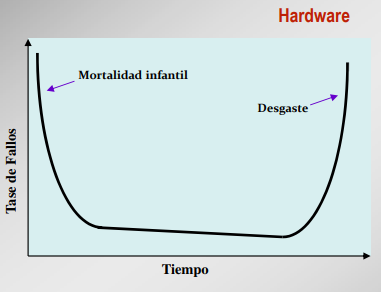
\includegraphics[scale=1,width=0.8\textwidth]{fallos_causados_hardware.png}
\end{figure}

\begin{figure}[h]
\centering
\label{tasa_software}
\caption{Evolución de la tasa de fallos debidos al software en el tiempo}
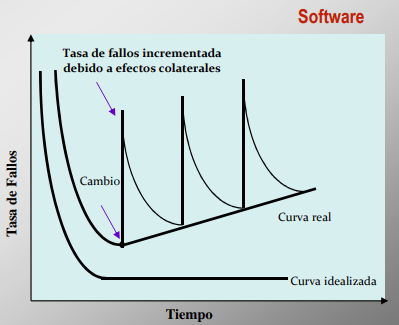
\includegraphics[scale=1,width=0.8\textwidth]{fallos_causados_software.png}
\end{figure}

\subsection{Tipos y dominios de aplicación del software}
\begin{itemize}
\item Software genérico. Sistema autónomo producido por una organización de desarrollo y vendido en el mercado abierto a cualquier cliente que pueda comprarlo.

\item Software a medida. Sistema desarrollado por una empresa especialmente para un cliente particular.

\end{itemize}

\textbf{Dominios de aplicación del software.} Actualmente, hay siete grandes categorías de software de computadora que plantean retos continuos a los ingenieros de software:

\begin{itemize}
\item Software de sistemas. Conjuntos de programas que proporcionan servicio a otros programas. Determinado software de sistemas (por ejemplo, compiladores, editores ,etc.) procesa estructuras de información complejas pero deterministas. Otras aplicaciones de sistemas (por ejemplo, componentes de sistemas operativos, manejadores, software de redes, procesadores de telecomunicaciones) procesan sobre todo datos indeterminados. En cualquier caso, el área de software de sistemas se caracteriza por: gran interacción con el hardware de la computadora, uso intensivo por parte de usuarios múltiples, operación concurrente que requiere la secuenciación, recursos compartidos y administración de un proceso sofisticado, estructuras complejas de datos e interfaces externas múltiples.

\item Software de aplicación. Programas que resuelven una necesidad específica de negocios. Las aplicaciones en esta área procesan datos comerciales o técnicos en una forma que facilita las operaciones de negocios o la toma de decisiones administrativas o técnicas. Además de las aplicaciones convencionales de procesamiento de datos, el software de aplicación se usa para controlar funciones de negocios en tiempo real (por ejemplo, procesamiento de transacciones en punto de venta).

\item Software de ingeniería y ciencias. Implementa algoritmos ``devoradores'' de números. Las aplicaciones van de la astronomía a la vulcanoogía, del análisis de tensiones en automóviles a la dinámica orbital del transbordador espacial, y de la biología molecular a la manufactura automatizada. Sin embargo, las aplicaciones modernas dentro del área de la ingeniería y las ciencias están abandonando los algoritmos númericos convencionales. El diseño asistido por computadora, la simulación de sistemas y otras aplicaciones interactivas, han comenzado a hacerse en tiempo real e incluso han tomado características del software de sistemas. 

\item Software empotrado. Reside dentro de un producto o sistema e implementa y controla características y funciones para el usuario final y para el sistema en sí. Ejecuta funciones limitadas y particulares (por ejemplo, control del tablero de un horno de microondas) o provee una capacidad significativa de funcionamiento y control (funciones digitales en un automovil, como el control del combustible, el tablero de control y de los sistemas de frenado).

\item Software de gestión. Proporciona una capacidad específica para uso de mucho consumidores diferentes. Se centra en algún mercado limitado y particular o se dirige a mercados masivos de consumidores.

\item Aplicaciones Web. llamadas ``webapps'', esta categoría de software centrado en redes agrupa una amplia gama de aplicaciones. En su forma más sencilla, las webapps son poco más que un conjunto de archivos de hipertexto vinculados que presentan información con uso de texto y gráficas limitadas. Sin embargo, desde que surgió Web 2.0, las webapps están evolucionando hacia ambientes de cómputo sofisticados que no sólo proveen características aisladas, funciones de cómputo y contenido para el usuario final, sino que también están integradas con bases de datos corporativas y aplicaciones de negocios.

\item Software de inteligencia artificial. Implementa algoritmos no numéricos para resolver problemas complejos difíciles de tratar computacionalmente o con análisis directo. Las aplicaciones en este área incluyen la robótica, sistemas expertos, reconocimiento de patrones, redes neurales artificiales, demostración de teoremas y juegos.
\end{itemize}

\subsection{Proceso de producción}

\begin{figure}[h]
\centering
\caption{Proceso de producción del software}
\includegraphics[scale=1,width=0.8\textwidth]{proceso_producción.png}
\end{figure}

\begin{itemize}
\item Definición. Se debe realizar ingeniería de sistemas, ingeniería de requisitos y planificación de proyectos.

\item Construcción. Se debe realizar diseño del software, generación del código y prueba del software.

\item Evolución. Se debe realizar corrección, adaptación, mejor y prevención.
\end{itemize}

\subsection{Efuerzo requerido por etapas}
\begin{figure}[h]
\centering
\caption{Esfuerzo requerido por etapas}
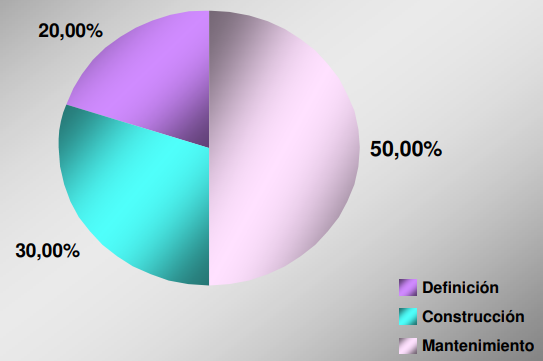
\includegraphics[scale=1,width=0.8\textwidth]{esfuerzo_requerido.png}
\end{figure}

\begin{figure}
\centering
\caption{Mantenimiento}
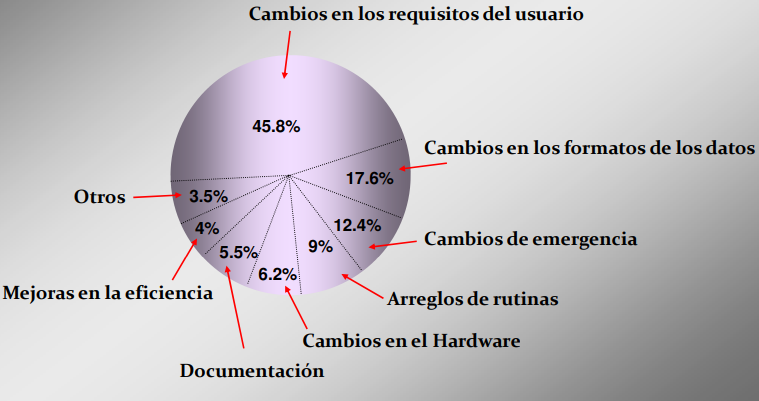
\includegraphics[scale=1,width=0.8\textwidth]{mantenimiento.png}
\end{figure}

\subsection{Problemas}
En el desarrollo del software pueden ocurrir varios tipos de problemas distintos.

\begin{itemize}
\item Comunicación entre personas, bien sea entre los desarrolladores y los clientes o directamente entre los desarrolladores.

\item Incumplimiento de la planificación. Normalmente los plazos de entrega son decididos por directivos que realmente no conocen el tiempo requerido en el desarrollo de un proyecto. Cuando se acerca la fecha límite y ante el miedo de perder a un cliente importante es común contratar más personal con el fin de terminar el proyecto a tiempo, esta práctica se conoce como ``horda mongoliana'', y lo normal es que en vez de ayudar perjudica. Esto se debe a que más medios son más difíciles de gestionar y al incorporar una persona nueva al equipo de desarrollo tendrá que aprender como se trabaja en la empresar, ponerse al día con los procedimientos, familiarizarse con el proyectos, etc. Finalmente la solución solamente hace más grande el problema.

\item Incorporar cambios en etapas avanzadas del proceso. Cuanto más se haya avanzado en el proyecto mayor será el coste de introducir cambios en el mismo.

\begin{figure}[h]
\centering
\caption{Coste de introducir cambios según la etapa}
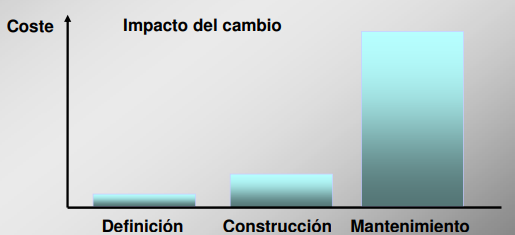
\includegraphics[scale=1,width=0.8\textwidth]{introducir_cambios.png}
\end{figure}
\end{itemize}

\section{El concepto de ingeniería del software}
La ingeniería del software se propuso por primera vez en 1968 en una conferencia en la que se habló sobre `a crisis del software''. Se volvió claro que las aproximaciones individuales al desarrollo de progamas no escalarían hasta sistemas software grandes y complejos. Estas no eran confiables, costaban más de lo esperado, se entregaban con retraso, eran difíciles de mantener y muy complejas y el software era de pobre ejecución. \\

Se concluyó que se debía entender el problema antes de desarrollar una aplicación. El diseño pasaba se convirtión en un actividad crucial, ya que el software debía tener alta calidad y ser fácil de mantener. Para conseguir esto se debía utilizar la ingeniería del software. \\

Durante los años setena y ocheta, una variedad de nuevos métodos y técnicas de ingeniería del softwere fueron desarrollados, tales como la programación estructurada, la ocultación de información y el desarrollo orientado a objetos. Se desarrollaron herramientas y notaciones estándar que actualmente son ampliamente usadas.

\subsection{Definición de Ingeniería del software}
\textbf{Definiciones:}

\begin{itemize}
\item ``Establecimiento y uso de principios fundamentales de la ingeniería con objeto de desarrollar en forma económica software que sea fiable y que trabaja en máquinas reales'' (Friz Bauer, 1972).

\item ``Aplicación práctica del conocimiento científico en el diseño y construcción de programas de computadora y la documentación asociada yrequerida para el desarrollo, operación y mantenimiento del programa'' (B. Bohem, 1976).

\item ``Aplicación de un enfoque sistemático, disciplinado y cuantificable al desarrollo, operación y mantenimiento del software; es decir, aplicación de la ingeniería del software'' (estándar - IEEE, 1993).
\end{itemize}

\subsection{Terminología usada en ingeniería del software}
\begin{itemize}
\item Sistema. Conjunto de elementos relacionados entre sí y con el medio, que forman una unidad o un todo organizativo.

\item Sistema basado en computadora. Conjunto o disposición de elementos organizados para cumplir una meta predefinida al procesar información.

\begin{figure}[h]
\centering
\caption{Esquema de sistema basado en computadora}
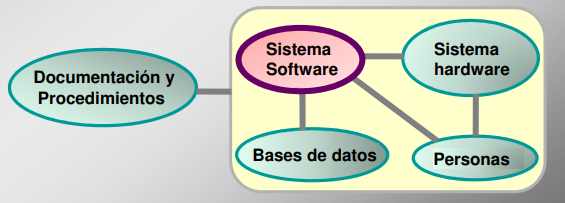
\includegraphics[scale=1,width=0.8\textwidth]{ejemplo_sistema_computadora.png}
\end{figure}

\item Sistema software. Conjunto de piezas o elementos software relacionados entre sí y organizados en subsistemas.

\begin{figure}
\centering
\caption{Esquema de sistema software}
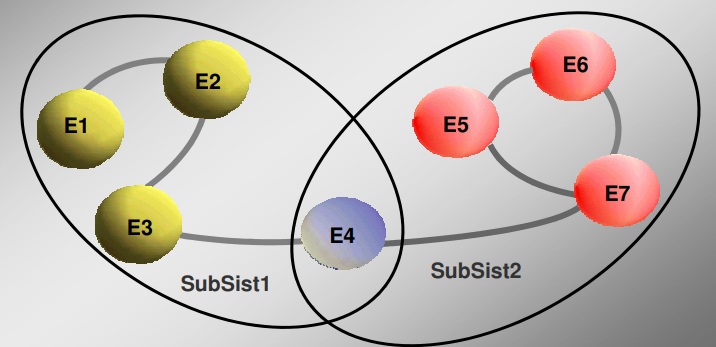
\includegraphics[scale=1,width=0.8\textwidth]{sistema_software.png}
\end{figure}

\item Modelos. Representación de un sistema en un determinado lenguaje: de un mismo sistema se pueden construir muchos modelos.

\item Principios. Elementos adquiridos mediante el conocimiento, que definen las características que debe poseer un modelo para ser una representación adecuada de un sistema.

\item Herramientas. Instrumentos que permiten la representación de modelos.

\item Técnicas. Modo de utilización de las herramientas.

\item Heurísticas. Conjunto de reglas empíricas, que al ser aplicadas producen modelos que se adecuan a los principios.

\item Métodos. Secuencia de actividades para la obtención de un producto (modelo), que describen cómo usar las herramientas y las heurísticas.
\end{itemize}

\subsection{Resumen}
\begin{figure}[h]
\centering
\caption{Resumen terminología software}
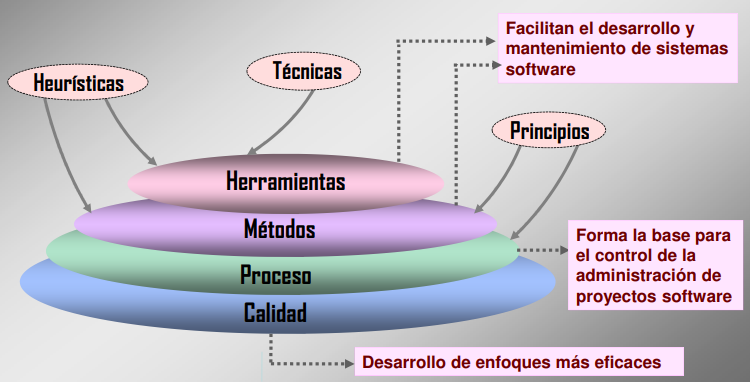
\includegraphics[scale=1,width=0.8\textwidth]{resumen.png}
\end{figure}

\begin{itemize}
\item \textbf{Modelos de ciclo de vida del software:}

	\begin{itemize}
	\item El modelo en cascada.
	\item Desarrollo incremental.
	\item Ingeniería del software orientada a la reutilización
	\end{itemize}
	
\item \textbf{Modelos orientados al cambio}
	
	\begin{itemize}
	\item Prototipo del sistema.
	\item Entrega incremental.
	\item Proceso unificado.
	\item Métodos ágiles.
	\end{itemize}
\end{itemize}

\begin{itemize}
\item Proceso de desarrollo o ciclo de vida del software. Estrategia que define la división y ubicación temporal de las etapas (o actividades) que se realizan durante el desarrollo del software.

\item Etapas. Se caracterizan por las tareas que se realizan por el producto (documento, artefacto, ...) que se obtiene.

\item Modelos (o paradigmas) de ciclo de vida del software. Son representaciones abstractas (simplificadas) del proceso de desarrollo del software.
\end{itemize}

Existen diversos modelos segń las etapas que se consideren, posición relativa de las mismas y las tareas a realizar en ellas.

\begin{thebibliography}{99}
\bibitem I. Sommerville. Software Engineering. Addison Wesley, 2011, ISBN 13: 978-0-13-703515-1
\bibitem R. Pressman. Ingeniería del Software. McGraw Hill, 2010, ISBN: 978-607-15-0314-5
\end{thebibliography}


\end{document}